\subsection{Question 1}

\subsubsection{Point 1}

\begin{equation}
	\begin{aligned}
		f(x) &= \frac{1}{C - x} + x\\
		f(2) &= 1\\
		1 &= \frac{1}{C - 2} + 2\\
		C &= 1
	\end{aligned}
\end{equation}

Pour que l'IVP soit stable, il faut que $\frac{\delta F}{\delta f}|_{(x_i, \zeta_i)}<0$

\begin{equation}
	\begin{aligned}
		\frac{\delta F}{\delta f}|_{(x_i, \zeta_i)} &= \frac{\delta}{\delta f} (1+(x-f(x))^2)\\
		&= (2f(x)-2x)|_{(x_i, \zeta_i)}\\
		(2f(x)-2x) &<0\\
		f(x)-x &< 0\\
		\frac{1}{1-x}+x-x&<0
	\end{aligned}
\end{equation}

Si on vérifie cette dernière inéquation pour tous les $x$ d'intéret (à savoir $x \geq 2$), on constate qu'elle est toujours vérifiée. L'IVP est donc stable pour les valeurs d'intérêt.

\subsubsection{Point 2}

\begin{equation}
	\begin{aligned}
		f_2 &= 1\\
		f_{i+1} &= h(1 + (x_i - f_i)^2)+f_i\\
	\end{aligned}
\end{equation}

Pour que les itérations soient stable, il faut que $h < \frac{-2}{\frac{\delta F}{\delta f}|_{(x_i, \zeta_i)}}$

\begin{equation}
	\begin{aligned}
		h &< \frac{-2}{\frac{\delta F}{\delta f}|_{(x_i, \zeta_i)}}\\
		&< \frac{-2}{2f(x)-2x}\\
		&< \frac{-1}{f(x)-x}\\
		&< \frac{-1}{\frac{1}{1-x}+x-x}\\
		&< x-1
	\end{aligned}
\end{equation}

Il faut donc choisir un $h$ plus petit que $1$ pour que les itérations soient stable.

\subsubsection{Point 3}

\code{littleclasses}{ForwardEuler.java}

Pour adapter le code à une autre fonction, il faut modifier les variables dans la méthode \texttt{main} ainsi que la méthode \texttt{F}. Il est également possible de mettre la fonction exacte dans la méthode \texttt{exactFunction} et de mettre alors le booléen \texttt{compareWithExactFunction} à \texttt{true}. Dans ce cas, le tableau renvoyé par la méthode \texttt{process} contiendra une troisième colonne avec les évaluations pour ces $x$ de la fonction exacte. On peut alors créer un graphe pour comparer les résultats obtenus par Forward Euler et les valeurs exactes avec gnuplot par exemple via la commande suivante :

\begin{lstlisting}
plot 'forward_euler.txt' using 1:2 with lines title 'Forward Euler', '' using 1:3 with lines title 'Exact function'
\end{lstlisting}

\begin{figure}[H]
	\caption{\label{12_forward_1} Forward Euler avec $h=0.25$}
	\centering
	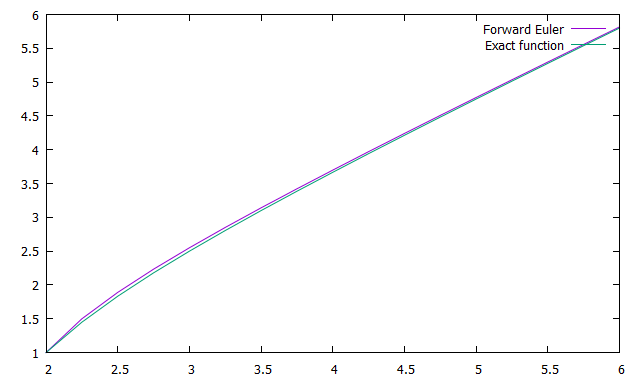
\includegraphics[scale = 0.6]{12_forward_1.png}
\end{figure}


\subsection{Question 2}

\begin{equation}
	\begin{aligned}
	\begin{cases}
	f'(x) = x + \sqrt{f(x)}\\
	f(1) = 2
	\end{cases}
	\end{aligned}
\end{equation}

Pour l'implémentation de Forward Euler, il nous suffit d'adapter l'implémentation de la question précédente en modifiant les variables de la valeur initiale et la méthode \texttt{F}. Pour le Classical Runge-Kutta on peut très simplement l'implémenter en se basant sur la structure de notre implémentation pour Forward Euler.

\code{littleclasses}{RK4.java}

\subsubsection{Point 1}

// TO DO

\subsubsection{Point 2}

Pour calculer le plus grand $h$ qui nous permette d'obtenir une solution exacte arrondie à 4 décimales, on peut utiliser une boucle qui commence avec un grand $h$ et le réduit tant que la différence entre la solution obtenue et le solution exacte est trop grande. Cette technique a été implémentée dans la méthode \texttt{calculate\_biggest\_h} et on peut ainsi déterminer que le plus grand $h$ qui nous permets d'obtenir une solution exacte est $0.2$.

\subsubsection{Point 3}

// TO DO

\subsection{Question 3}

\begin{equation}
	\begin{aligned}
	\begin{cases}
	f'(x) = sin(f(x))\\
	f(0) = 1
	\end{cases}
	\end{aligned}
\end{equation}

\begin{equation}
	\begin{aligned}
		f(x_{i+1}) \approx f_{i+1} &= hF(x_{i+1}, f_{i+1}) + f_i\\
		&= h\cdot sin(f_{i+1}) + f_i
	\end{aligned}
\end{equation}
// TO DO

\subsection{Question 4}

\subsubsection{Point 1}

// TO DO

\subsubsection{Point 2}

// TO DO